\documentclass[10pt]{article}
\usepackage[margin=1in]{geometry}
\usepackage{jheppub} % for details on the use of the package, please see the JINST-author-manual
% page formatting
\usepackage{fancyhdr}
\pagestyle{fancy}

\renewcommand{\sectionmark}[1]{\markright{\textsf{#1}}}
\renewcommand{\subsectionmark}[1]{}
\lhead{\textbf{\thepage} \ \ \nouppercase{\rightmark}}
\chead{}
\rhead{}
\lfoot{}
\cfoot{}
\rfoot{}
\setlength{\headheight}{14pt}

\linespread{1.03} % give a little extra room
\setlength{\parindent}{0.2in} % reduce paragraph indent a bit
\setcounter{secnumdepth}{2} % no numbered subsubsections
\setcounter{tocdepth}{2} % no subsubsections in ToC
\usepackage{lineno}
\usepackage{amsmath,amsthm,amsfonts,amssymb,amscd,physics,cancel,mathtools}
\usepackage{tcolorbox}
\usepackage{marginnote,tensor}
\usepackage[spanish]{babel}
%~~~~~~~~~ Document setup
% \usepackage[spanish]{babel} % English formatting
\usepackage[utf8]{inputenc} % Standard encoding
% \usepackage[a4paper,left=3cm,bottom=3cm]{geometry} % Page formatting
\usepackage{indentfirst} % Indents the first paragraph
\usepackage{amsmath} % Maths type package
\usepackage{bm} % Bold font maths
\usepackage{graphicx} % Advanced graphics package
\usepackage[export]{adjustbox} 
\usepackage{pdflscape} % Make pages landscape
\usepackage{fancyhdr} % Fancy headers
% \usepackage[colorlinks=true,citecolor=blue,urlcolor=blue,linkcolor=black]{hyperref} % Link colours
%\usepackage{natbib} % Bibliography
% \usepackage{flafter} % Reference any 'float'
% \usepackage[framemethod=tikz]{mdframed} % Box off stuff
\usepackage{color} % Colour support
\usepackage{wrapfig} % Text flowing around figures
\usepackage{lipsum} % Generates meaningless text
\usepackage{xcolor}
%\usepackage{biblatex}
%\usepackage[backend=bibtex]{biblatex}
%\addbibresource{bibliography.bib}
%\hypersetup{colorlinks=true, linkcolor=blue}


\theoremstyle{definition}
\newtheorem{ej}{Ejemplo}[section]
\newtheorem{teor}{Teorema}[section]
\newtheorem{sol}{Solución}[section]
\newtheorem{dem}{Demostración}[section]
\newtheorem{cor}{Corolario}[section]
\newtheorem{post}{Postulado}
\newtheorem{prop}{Propiedad}[section]
\newtheorem{prueba}{Prueba}[section]
\newtheorem{problema}{Problema}[section]

\def\a{\alpha}
\def\b{\beta}
\def\g{\gamma}
\def\G{\Gamma}
\def\d{\delta}
%\def\D{\Delta}
%\def\e{\eta}
\def\la{\lambda}
\def\La{\Lambda}
\def\k{\kappa}
\def\m{\mu}
\def\n{\nu}
\def\r{\rho}
\def\p{\rho}
\def\o{\omega}
\def\s{\sigma}
\def\S{\Sigma}
\def\t{\tau}
\def\p{\pi}
\def\f{\phi}
\def\vf{\varphi}
\def\ep{\epsilon}
\def\th{\theta}
\def\Th{\Theta}
\def\z{\zeta}
\def\zc{Z_{\rm C}}
\def\zgc{Z_{\rm GC}}
\def\zp{Z_{p}}
\def\ogc{\omega_{\rm GC}}
\def\Ogc{\Omega_{\rm GC}}
\def\dst{\dd S_{\rm total}}
\def\vec{\vb*}
\def\eb{e^{-\beta E_i}}
\def\ebep{e^{-\beta \epsilon_i}}
\def\eba{e^{-\beta E_i-\alpha Q_i}}
\def\ebaj{e^{-\beta E_j-\alpha Q_j}}
\newcommand{\summ}{\sum_{i=1}^m}
\newcommand{\sumi}{\sum_i}
\newcommand{\sumj}{\sum_j}
\def\var{\text{Var}}
\def\intpq{\int\frac{\dd^3\vec{p}\dd^3\vec{q}}{(2\pi\hbar)^3}}
\def \sumn1 {\sum_{n=1}^\infty}
\def\ebem{e^{-\b (\ep-\m )}}


%-----COLORS LIST ------
\definecolor{azure(colorwheel)}{rgb}{0.0, 0.5, 1.0}
\definecolor{DarkViolet}{RGB}{148,0,211}
\definecolor{myDarkBlue}{rgb}{0,0.1,0.7}
\definecolor{DarkBlue}{RGB}{0,0,153}
\definecolor{amber}{rgb}{1.0, 0.49, 0.0}
\definecolor{amaranth}{rgb}{0.9, 0.17, 0.31}
\definecolor{nicered}{rgb}{0.7,0.1,0.1}
\definecolor{brown}{rgb}{0.5,0.1,0.1}
\definecolor{nicegreen}{rgb}{0.0,0.3,0.0}
\definecolor{tealgreen}{rgb}{0.0, 0.51, 0.5}
\def\red#1{{\color{red} #1}}
\def\green#1{{\color{green} #1}}
\def\blue#1{{\color{blue} #1}}
\def\orange#1{{\color{orange} #1}}
%----------------------
\newcommand{\mycolor}{DarkViolet}
\def\myColor#1{{\color{\mycolor} #1}}
\definecolor{tclr}{RGB}{148,0,211}
%----------------------
\newcommand{\corr}[1]{\textcolor{nicered}{#1}}
\newcommand{\nick}[1]{\textcolor{olive}{#1}}
\newcommand{\teo}[1]{\textcolor{azure(colorwheel)}{#1}}
\newcommand{\chteo}[2]{\corr{\st{#1}} \teo{(#2)}}
\newcommand{\bako}[1]{\textcolor{DarkViolet}{#1}}
\newcommand{\than}[1]{\textcolor{magenta}{#1}}
%----------------------
\usepackage{hyperref}
\hypersetup{colorlinks,bookmarksopen,
	bookmarksnumbered,
	citecolor={nicered},
	linkcolor={myDarkBlue},
	urlcolor={tealgreen},
	pdfstartview=FitH}





% \arxivnumber{1234.56789} % if you have one

%\title{\boldmath Mecánica Estadística}

% Collaborations

%% [A] If main author
%% \collaboration{\includegraphics[height=17mm]{collabroation-logo}\\[6pt]
%%  XXX collaboration}

%% or
%% [B] If "on behalf of"
%% \collaboration[c]{on behalf of XXX collaboration}


% Authors
% The "\note" macro will give a warning: "Ignoring empty anchor...", you can safely ignore it.

%% [A] simple case: 2 authors, same institution
%% \author[1]{A. Uthor\note{Corresponding author.}}
%% \author{and A. Nother Author}
%% \affiliation{Institution,\\Address, Country}

%% or, e.g.
%% [B] more complex case: 4 authors, 3 institutions, 2 footnotes
%% \author[a,b]{F. Irst,\note{Now at another university}}
%% \author[c]{S. Econd,}
%% \author[a,2]{T. Hird\note{Also at Some University.}}
%% \author[c,2]{and Fourth}
%% \affiliation[a]{Institution_1,\\Address, Country}
%% \affiliation[b]{Institution_2,\\Address, Country}
%% \affiliation[c]{Institution_3,\\Address, Country}

\author{Borja Diez}
\affiliation{Universidad Arturo Prat}
% \affiliation{Another University,\\
% different-address, Country}

% E-mail addresses: only for the corresponding author
\emailAdd{borjadiez1014@gmail.com}

\abstract{Notas sobre Mecánica Estadistica }



\begin{document}
% make title page
\thispagestyle{empty}
\bigskip \
\vspace{0.1cm}

\begin{center}
{\fontsize{22}{22} \selectfont\bf \sffamily  Mecánica Estadística}
\vskip 16pt
{\fontsize{36}{36} \selectfont \bf \sffamily Tarea 01}
\vskip 24pt
{\fontsize{18}{18} \selectfont \rmfamily Borja Diez} 
\vskip 6pt
%{\fontsize{14}{14} \selectfont \ttfamily borjadiez1014@gmail.com}
\vskip 6pt
{\fontsize{14}{14} \selectfont  \sffamily \today}
\vskip 24pt
\end{center}

%Estas notas de clase están basadas en el curso dictado por el \href{https://inspirehep.net/authors/1318424?ui-citation-summary=true}{Dr. Ignacio Araya} durante el primer semestre del año 2024 en la Universidad Arturo Prat y han sido escritas con propósito de estudio personal.
%
%Las notas están divididas por clase. Adicionalmente han sido complementadas con desarrollos de cálculo personal y comentarios sacados principalmente de \textcolor{blue}{Lecture notes on statistical mechanics} de \href{https://inspirehep.net/authors/992816}{Scott Pratt}. 

\underline{Nota}: Para los ejercicios del capítulo 2, primero hice el Problema \ref{prob:2.7} (Problema 2.7 del libro), así que recomiendo revisar ese primero y luego los otros dos restantes correspondientes a ese capítulo ya que hay cálculos similares que están mejor explicados en este problema.
 



% make table of contents
\newpage
\tableofcontents
\newpage

\section{Problema 1.3}

\begin{tcolorbox}
\begin{problema}
	Considere dos fermiones idénticos (ningún nivel de energía puede tener más de una partícula) en un sistema de $2$ niveles de energía, donde las energías son $0$ y $\epsilon$. En términos de $\epsilon$ y $T$ calcular
	\begin{enumerate}
		\item La función partición del ensamble canónico $\zc$
		\item La energía promedio $\ev{E}$. Además ver que sucede con $\ev{E}$ en los límites cuando $T\to 0$ y $T\to\infty$.
		\item La entropía $S$. Analizar los mismo límites para $T$.
		\item Ahora, el sistema es conectado a un baño de partículas con potencial químico $\m$. Calcule $\zgc(\m,T)$. Encuentre el número  de partículas, $\ev{N}$ como función de $\m$ y $T$. Además, calcules los mismo límites anteriores en $T$.
	\end{enumerate}
\end{problema}
\end{tcolorbox}

\begin{sol}
\
\begin{enumerate}
\begin{figure}[h!]
	\centering
	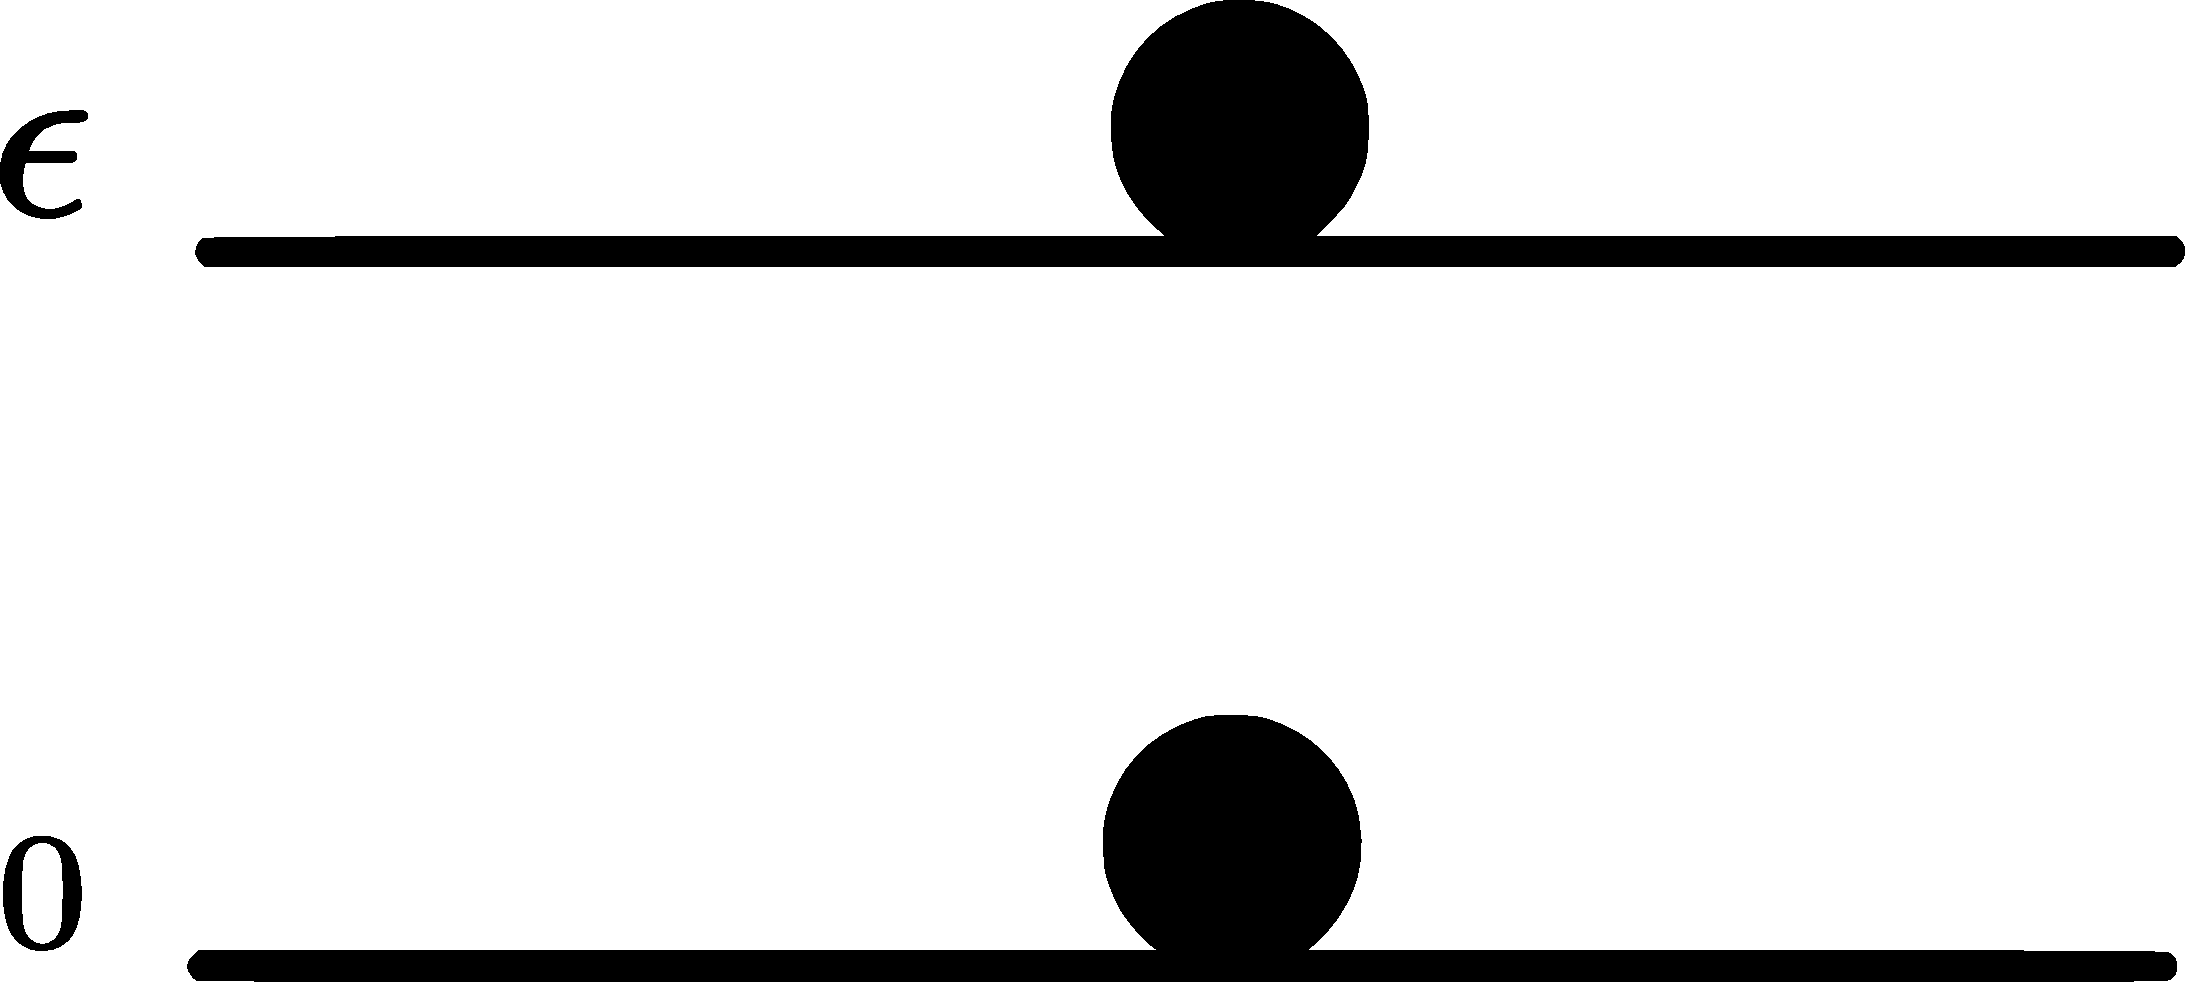
\includegraphics[scale=0.13]{energy-levels.pdf}
	\caption{Única configuración posible para el problema dado.}
	\label{fig:1.3}
\end{figure}	
\item 
Notemos que debido al hecho de que estamos considerando $2$ fermiones idénticos en un sistema de $2$ niveles de energía, existe sólo una configuración posible para el sistema, de manera tal que ningún nivel de energía tengas más de una partícula, representada en la Figura \ref{fig:1.3}.

Sabemos que la función de partición del ensamble canónico viene dada por
\begin{equation}
  \zc=\sumi e^{-\b \epsilon_i},\qquad \b=\frac{1}{\k T}
\end{equation}
Para este caso, tenemos
\begin{align}
  \zc&=e^{-\b \epsilon}\\
 \Aboxed{ \zc&=e^{-\epsilon/\k T}\label{1-Zc}}
\end{align}

\item 
La energía promedio se obtiene como
\begin{align}\label{13-evE}
  \ev{E}=\sumi \epsilon_iP_i
\end{align}
donde
\begin{equation}
	P_i=\frac{e^{-\b \epsilon_i}}{\zc }
\end{equation}
Usando \eqref{1-Zc}, se tiene
\begin{equation}
  P_i=\frac{e^{-\b \epsilon}}{e^{-\b \epsilon}}=1
\end{equation}
así de \eqref{13-evE} , la energía promedio es
\begin{equation}\label{E}
\boxed{  \ev{E}=\epsilon}
\end{equation}
Notemos que esta igual puede ser calculada usando
\begin{align}
  \ev{E}&=-\pdv{\b}\ln (\zc)\\
  &=-\pdv{\b}\ln(e^{-\b \epsilon})\\
  &=-\pdv{\b}(-\b \epsilon)\\
  &=\epsilon
\end{align}
lo cual es consistente con \eqref{E}. Notemos que este valor no depende de $T$, luego
\begin{equation}
  \boxed{\lim_{T\to 0}\ev{E}= \lim_{T\to\infty}\ev{E}=\epsilon}
\end{equation}
Es decir, para cualquier $T$, el valor de expectación de la energía será el mismo. Pero esto es consistente ya que el sistema siempre estará en la única configuración en la cual puede estar, con energía total $\epsilon$.
% todas las configuraciones tienen la misma probabilidad, pero sólo existe una única configuración posible. Luego, el resultado es consistente.

\item 
Para calcular la entropía $S$, notemos que de la energía libre de Hemholtz,
\begin{equation}
  F=\ev{E}-TS=-\k T\ln (\zc)
\end{equation}
podemos despejar $S$,
\begin{equation}
  S=\frac{\ev{E}}{T}+\k \ln(\zc )
\end{equation}
Usando lo encontrado anteriormente, tenemos
\begin{align}
  S&=\frac{\epsilon}{T}+\k (-\b \epsilon)\\
  &=\frac{\epsilon}{T}-\frac{\kappa}{\k T}\epsilon\\
  &=\frac{\epsilon}{T}-\frac{\epsilon}{T}\\
  \implies \Aboxed{S&=0}
\end{align}
Al igual que antes este valor no depende de $T$, luego
\begin{equation}
  \boxed{\lim_{T\to 0}S= \lim_{T\to\infty}S=0}
\end{equation}
Este resultado igual es consistente con lo esperado, ya que al existir sólo un único microestado comptible con  el sistema, $S\sim \ln (1)=0$, independientmenete del valor de $T$.
 %--------0--------
 \item
Debido a que ahora estamos permitiendo que el número de partículas fluctúe, debemos calcular la función partición del ensamble gran canónico $\zgc$ de manera similar al ejercicio realizado en clases para el caso de los bosones. Por definición, $\zgc$ viene dada por
\begin{equation}\label{1.zgc}
  \zgc=\sum_le^{-\b (E_l-\m N_l)}
\end{equation}
donde $l$ es la configuración total del sistema, $E_l$ es la energía total del sistema y $N_l$ corresponde al número de partículas total del sistema. Sea $i$ el número de partículas en el nivel $1$ con energía $0$ y sea $j$ el número de partículas en el nivel $2$ con energía $\epsilon$. Así, se tiene
\begin{align}
  E_l&=0\cdot i+\epsilon\cdot j=\epsilon j\\
  N_l&=i+j
\end{align}
Notar que en este caso, debido a que estamos considerando fermiones, el número de partículas que puede haber en un nivel de energía puede ser únicamente $0$ ó $1$. Luego, \eqref{1.zgc} queda
\begin{align}
  \zgc &=\sum_{i,j}e^{-\b(\epsilon j-\m i-\m j)}\\
  &=\sum_{i=0}^1e^{\b \m i}\sum_{j=0}^1e^{-\b (\epsilon-\m )j}\\
  &=\left(1+e^{\b \m }\right)\left(1+e^{-\b(\epsilon-\m )}\right)\label{1.zgc-exp}
\end{align}
\begin{equation}
	\implies\boxed{ \zgc=\left(1+e^{\m/\k T }\right)\left(1+e^{-(\epsilon-\m )/\k T}\right)}
\end{equation}

Para calcular el número de partículas, usamos
\begin{equation}\label{1.N}
  \ev{N}=-\pdv{\a}\ln(\zgc)=\pdv{(\b\m )}\ln(\zgc)
\end{equation}
De \eqref{1.zgc-exp} se tiene
\begin{align}
  \ln(\zgc)&=\ln \left[\left(1+e^{\b \m }\right)\left(1+e^{-\b(\epsilon-\m )}\right)\right]\\
  &=\ln\left(1+e^{\b \m }\right)+ \ln \left(1+e^{-\b(\epsilon-\m )}\right)
\end{align}
De \eqref{1.N}
\begin{align}
  \ev{N}&=\pdv{(\b\m )}\ln(\zgc)\\
  &=\pdv{(\b \m)  }\left[\ln\left(1+e^{\b \m }\right)+ \ln \left(1+e^{-\b(\epsilon-\m )}\right)\right]\\
  &=\frac{e^{\b\m }}{1+e^{\b \m }}+\frac{e^{-\b (\epsilon-\m )}}{1+e^{-\b(\epsilon-\m )}}
\end{align}
\begin{equation}
	\implies 	\boxed{\ev{N}=\frac{e^{\m/\k T }}{1+e^{ \m/\k T }}+\frac{e^{-(\epsilon-\m )/\k T}}{1+e^{-(\epsilon-\m )/\k T}}}
\end{equation}

Para calcular los límites notemos que para $T\to 0$ habrá una indeterminación tipo $\infty	/\infty$, luego, usamos L'Hopital,
\begin{align}
  \lim_{T\to 0 }\ev{N}&=\lim_{T\to 0}\left\{\frac{e^{\m/\k T }}{1+e^{ \m/\k T }}+\frac{e^{-(\epsilon-\m )/\k T}}{1+e^{-(\epsilon-\m )/\k T}}\right\}\\
  &=\lim_{T\to 0}\left\{\frac{-\dfrac{\m }{\k T^2}e^{\m/\k T}}{-\dfrac{\m }{\k T^2}e^{\m/\k T}}+\frac{\dfrac{k}{T^2}(\epsilon-\m )e^{-(\epsilon-\m )/\k T}}{\dfrac{k}{T^2}(\epsilon-\m )e^{-(\epsilon-\m )/\k T}}\right\}\\
  &=\lim_{T\to 0}\{1+1\}\\
  &=\lim_{T\to 0}\left\{2\right\}\\
  &=2
\end{align}

Por otro lado,
\begin{align}
  \lim_{T\to \infty }\ev{N}&=\lim_{T\to\infty }\left\{\frac{e^{\m/\k T }}{1+e^{ \m/\k T }}+\frac{e^{-(\epsilon-\m )/\k T}}{1+e^{-(\epsilon-\m )/\k T}}\right\}\\
  &=\frac{1}{1+1}+\frac{1}{1+1}\\
  &=\frac{1}{2}+\frac{1}{2}\\
  &=1
\end{align}
\end{enumerate}
%TODO interpretación

















\end{sol}

\newpage
\section{Problema 1.5}
\begin{tcolorbox}
\begin{problema}
Asumiendo que la presión $P$ es independiente de $V$ cuando es escrita como función de $\m$ y $T$, es decir, $\ln\zgc=PV/\k T$ (lo cual es verdad si el sistema es mucho más grande que el rango de interacción),
\begin{enumerate}
	\item Encuentre expresiones para $E/V$ y $Q/V$ en términos de $P,T$ y derivadas parciales de $P$ o $P/T$ con respecto a $\a\equiv-\m/\k T$ y $\b\equiv 1/\k T$. Aquí, asuma que el potencial químico está asociado con el número conservado $Q$.
	\item Encuentre una expresión para $C_V=\eval{\dv*{E}{T}}_{Q,V}$ en términos de $P/T,E,Q,V$ y derivadas de $P,P/T,E$ y $Q$ con respecto a $\b$ y $\a$.
	\item Muestre que la densidad de entropía es $s=\eval{{\partial_T P}}_\m $.
\end{enumerate}
\end{problema}
\end{tcolorbox}

\begin{sol}
\begin{enumerate}
\
	\item 

	Dado que 
	\begin{equation}
  \ln(\zgc )=\frac{PV}{\k T}
\end{equation}
y sabemos que el valor de expectación de la energía en el ensamble gran canónico viene dado por
\begin{equation}
  \ev{E}=-\pdv{\b}\ln(\zgc )
\end{equation}
tenemos
\begin{align}
  \ev{E}&=-\pdv{\b}\left(\frac{PV}{\k T}\right)\\
  &=-V\pdv{\b}\left(\frac{P}{\k T}\right)
\end{align}
\begin{equation}\label{1-5-EV}
  \implies \boxed{\frac{\ev{E}}{V}=-\pdv{\b}\left(\frac{P}{\k T}\right)}
\end{equation}
pero además sabemos que $\b =1/\k T$. Luego, \eqref{1-5-EV} queda
\begin{equation}
  \frac{\ev{E}}{V}=-\pdv{\b}\left(P \b \right)
\end{equation}
\begin{equation}
  \implies \boxed{\frac{\ev{E}}{V}=-P}
\end{equation}

De manera similar, sabemos que el valor de expextación de $Q$ se relaciona con la función partición del ensamble gran canónico mediante
\begin{equation}
  \ev{Q}=-\pdv{\a }\ln(\zgc )
\end{equation}
así,
\begin{align}
  \ev{Q}&=-\pdv{\a}\left(\frac{PV}{\k T}\right)\\
  &=-V\pdv{\a}\left(\frac{P}{\k T}\right)
\end{align}
\begin{equation}\label{1-5-QV}
  \implies \boxed{\frac{\ev{Q}}{V}=-\pdv{\a}\left(\frac{P}{\k T}\right)}
\end{equation}
además,
\begin{equation}
  \a=-\frac{\m }{\k T}\implies \dd\a =\frac{\m }{\k T^2}\dd T\implies \pdv{\a}=\frac{\k T^2}{\m }\pdv{T}
\end{equation}
Reemplazando en \eqref{1-5-QV},
\begin{align}
  \frac{\ev{Q}}{V}&=-\frac{\k T^2}{\m }\pdv{T}\left(\frac{P}{\k T}\right)\\
  &=\frac{\k T^2}{\m }\frac{P }{\k }\frac{1}{T^2}
\end{align}
\begin{equation}
  \implies\boxed{ \frac{\ev{Q}}{V}=\frac{P}{\m }=-\frac{P}{\a\k T}}
\end{equation}
%%%%%%%%%%%%%%
\item 
El calor específico a volúmen constante viene dado por
\begin{equation}
  C_V=\eval{\dv{E}{T}}_{Q,V}
\end{equation}
Notemos que
\begin{equation}
  \b=\frac{1}{\k T}\implies \dd\b=-\frac{1}{\k T^2}\dd T\implies \dv{\b}=-\k T^2\dv{T}\implies \dv{T}=-\frac{1}{\k T^2}\dv{\b}
\end{equation}
Así, podemos escribir
\begin{equation}\label{1-5-CV}
  C_V=-\frac{1}{\k T^2}\eval{\dv{E}{\b }}_{Q,V}
\end{equation}
Para poder encontrar $\eval{\pdv*{E}{\b }}_{Q,V}$ notemos que la variación de la energía promedio $\ev{E}$ escrita en función de $\a$ y $\b$ viene dada por
\begin{equation}\label{1-5-dE}
  \d E=\pdv{E}{\a }\d \a +\pdv{E}{\b }\d \b 
\end{equation}
De manera similar, dado que estamos a $Q$ constante, se tiene que la variación de $Q=0$,
\begin{equation}
  \d Q=\pdv{Q}{\a }\d \a +\pdv{Q}{\b }\d \b =0
\end{equation}
\begin{equation}
  \implies \pdv{Q}{\a }\d \a=-\pdv{Q}{\b}\d\b 
\end{equation}
podemos despejar $\d\a$ a $Q$ constante,
\begin{equation}
  \implies \d\a =-\frac{\pdv*{Q}{\b }}{\pdv*{Q}{\alpha }}\d\b 
\end{equation}
Reemplazando en \eqref{1-5-dE},
\begin{align}
 \eval{\d E}_{Q,V}&=-\pdv{E}{\a }\frac{\pdv*{Q}{\b }}{\pdv*{Q}{\alpha }}\d\b +\pdv{E}{\b }\d \b \\
 &=\d\b\left[\pdv{E}{\b }-\pdv{E}{\a }\frac{\pdv*{Q}{\b }}{\pdv*{Q}{\alpha }}\right]
\end{align}
\begin{equation}
  \implies \eval{\dv{E}{\b }}_{Q,V}=\pdv{E}{\b }-\pdv{E}{\a }\frac{\pdv*{Q}{\b }}{\pdv*{Q}{\alpha }}
\end{equation}

Reemplazando en \eqref{1-5-CV},
\begin{align}
   C_V&=-\frac{1}{\k T^2}\eval{\dv{E}{\b }}_{Q,V}\\
   &=-\frac{1}{\k T^2}\left(\pdv{E}{\b }-\pdv{E}{\a }\frac{\pdv*{Q}{\b }}{\pdv*{Q}{\alpha }}\right)
\end{align}
pero,
\begin{equation}
  \b=\frac{1}{\k T}\implies \k \b^2=\frac{1}{\k T^2}
\end{equation}
Luego, $C_V$ escrito en términos de derivadas de $E$ y $Q$ con respecto a $\a$ y $\b$ queda,
\begin{equation}
 \boxed{ C_V=-\k\b^2\left(\pdv{E}{\b }-\pdv{E}{\a }\frac{\pdv*{Q}{\b }}{\pdv*{Q}{\alpha }}\right)}
\end{equation}


\item 
De la primera y la segunda ley de la termodinámica combinadas, se tiene
\begin{equation}
  \dd E=T\dd S-P\dd V+\m \dd N
\end{equation}
Podemos \textit{integrar por partes} a los diferenciales del lado derecho,
\begin{align}
  \dd E&=\dd (TS)-S\dd T-\dd(PV)+V\dd P+\dd(\m N)-N\dd\m
\end{align}
\begin{equation}
  \implies \dd E-\dd (TS)+\dd(PV)-\dd (\m N)=-S\dd T+V\dd P-N\dd\m 
\end{equation}
\begin{equation}
  \implies \dd (E-TS+PV-\m N)=-S\dd T+V\dd P-N\dd\m 
\end{equation}
Pero en clases vimos que la energía libre de Gibbs viene dada por
\begin{equation}
  G=\m N=E-TS+PV\implies E-TS+PV-\m N=0
\end{equation}
Así,
\begin{align}
  0&=-S\dd T+V\dd P-N\dd\m 
\end{align}
considerando $\m$ constante,
\begin{equation}
  S\dd T=V\dd P\implies \frac{S}{V}=\eval{\pdv{P}{T}}_\m 
\end{equation}
Finalmente, la densidad de entropía viene dada por
\begin{equation}
  \boxed{s=\eval{\pdv{P}{T}}_\m }
\end{equation}






























\end{enumerate}
\end{sol}
\newpage
\section{Problema 1.8}
\begin{tcolorbox}
\begin{problema}
	Comenzando con\begin{equation}
  T\dd S=\dd E+P\dd V-\m\dd Q,\quad \text{y}\quad  G\equiv E+PV-TS
\end{equation}
\begin{enumerate}
	\item Muestre que
	\begin{equation}
  S=-\eval{\pdv{G}{T}}_{N,P},\qquad V=\eval{\pdv{G}{P}}_{N,T}
\end{equation}
\item Comenzando con
 \begin{equation}\label{18-dS}
  \d S(P,N,T)=\pdv{S}{P}\d P+\pdv{S}{N}\d N+\pdv{S}{T}\d T
\end{equation}
Muestre que los calores específicos,
\begin{equation}
  C_P\equiv T\eval{\pdv{S}{T}}_{N,P},\qquad C_V\equiv T\eval{\pdv{S}{T}}_{N,V}
\end{equation}
satisfacen la relación:
\begin{equation}
  C_P=C_V-T\left(\eval{\pdv{V}{T}}_{P,N}\right)^2\left(\eval{\pdv{V}{P}}_{T,N}\right)^{-1}
\end{equation}
Notar que la compresibilidad, $\equiv -\pdv*{V}{P}$, es positiva (a menos que el sistema sea inestable), luego $C_P>C_V$.
\end{enumerate}
\end{problema}
\end{tcolorbox}

\begin{sol}
\
\begin{enumerate}
\item 
La energía libre de Gibbs viene dada por
	\begin{equation}
  G= E+PV-TS
\end{equation}
o en su forma diferencial
\begin{equation}\label{3.dG}
  \dd G=\dd E+V\dd P+P\dd V-S\dd T-T\dd S
\end{equation}
de la expresión de la primera y la segunda ley de la termodinámica combinadas, donde consideraremos $Q=N$, tenemos
\begin{equation}
  T\dd S=\dd E+P\dd V-\m\dd N
\end{equation}
reemplazando en \eqref{3.dG},
\begin{align}
  \dd G&=\cancel{\dd E}+V\dd P+\cancel{P\dd V}-S\dd T-\cancel{\dd E}-\cancel{P\dd V}+\m\dd N\\
  &=V\dd P-S\dd T+\m\dd N
\end{align}
pero además,
\begin{equation}
  \dd G=\eval{\pdv{G}{P}}_{T,N}\dd P+\eval{\pdv{G}{T}}_{P,N}\dd T+\eval{\pdv{G}{N}}_{T,P}\dd N
\end{equation}
comparando estas dos última expresiones, se tiene
que 
\begin{equation}\label{18-GTGP}
  \boxed{\eval{\pdv{G}{T}}_{P,N}=-S,\qquad \eval{\pdv{G}{P}}_{T,N}=V}
\end{equation}


\item
De \eqref{18-dS} podemos calcular $\eval{\dd S}_N$,
\begin{align}
  \d S(P,N,T)&=\eval{\pdv{S}{P}}_{T,N}\d P+\cancelto{0}{\eval{\pdv{S}{N}\d N}_{T,P}}+\eval{\pdv{S}{T}}_{P,N}\d T\\
  &=\eval{\pdv{S}{P}}_{T,N}\d P+\eval{\pdv{S}{T}}_{P,N}\d T \label{18-dd S}
\end{align}
Queremos encontrar una expresión para $C_V$. Notemos que a volumen y número de partículas constantes se tiene
\begin{align}
  0=\eval{\d V}_N&=\eval{\pdv{V}{P}}_{T,N}\d P+\eval{\pdv{V}{T}}_{P,N}\d T+\cancelto{0}{\eval{\pdv{V}{N}}_{T,P}\d N}\\
  &=\eval{\pdv{V}{P}}_{T,N}\d P+\eval{\pdv{V}{T}}_{P,N}\d T
\end{align}
\begin{equation}
  \implies \eval{\pdv{V}{P}}_{T,N}\d P=-\eval{\pdv{V}{T}}_{P,N}\d T
\end{equation}
\begin{equation}
  \implies \d P=-\eval{\pdv{V}{T}}_{P,N}\left(\eval{\pdv{V}{P}}_{T,N}\right)^{-1}\d T
\end{equation}
Reemplazando en \eqref{18-dd S},
\begin{align}
  \eval{\d S}_{N,V}&=\eval{\pdv{S}{P}}_{T,N}\left[-\eval{\pdv{V}{T}}_{P,N}\left(\eval{\pdv{V}{P}}_{T,N}\right)^{-1}\d T\right]+\eval{\pdv{S}{T}}_{P,N}\d T\\
  &=-\eval{\pdv{S}{P}}_{T,N}\eval{\pdv{V}{T}}_{P,N}\left(\eval{\pdv{V}{P}}_{T,N}\right)^{-1}\d T+\eval{\pdv{S}{T}}_{P,N}\d T\\
  &=\left[-\eval{\pdv{S}{P}}_{T,N}\eval{\pdv{V}{T}}_{P,N}\left(\eval{\pdv{V}{P}}_{T,N}\right)^{-1}+\eval{\pdv{S}{T}}_{P,N}\right]\d T
\end{align}
Luego,
\begin{align}
  \eval{\pdv{S}{T}}_{N,V}&=-\eval{\pdv{S}{P}}_{T,N}\eval{\pdv{V}{T}}_{P,N}\left(\eval{\pdv{V}{P}}_{T,N}\right)^{-1}+\eval{\pdv{S}{T}}_{P,N}
\end{align}
Multiplicando a ambos lados por $T$,
\begin{align}\label{18-casi}
  T\eval{\pdv{S}{T}}_{N,V}&=-T\eval{\pdv{S}{P}}_{T,N}\eval{\pdv{V}{T}}_{P,N}\left(\eval{\pdv{V}{P}}_{T,N}\right)^{-1}+T\eval{\pdv{S}{T}}_{P,N}\\
  C_V&=-T\eval{\pdv{S}{P}}_{T,N}\eval{\pdv{V}{T}}_{P,N}\left(\eval{\pdv{V}{P}}_{T,N}\right)^{-1}+C_P
\end{align}
Además, podemos obtener una relación de Maxwell utilizando \eqref{18-GTGP}. Usando el hecho que
\begin{align}
  \pdv{G}{T}{P}&=\pdv{G}{P}{T}\\
  \left(\pdv{T}\left(\pdv{G}{P}\right)_{T,N}\right)_{P,N}&=\left(\pdv{P}\left(\pdv{G}{T}\right)_{P,N}\right)_{T,N}\\
  \eval{\pdv{V}{T}}_{P,N}&=-\eval{\pdv{S}{P}}_{N,T}
\end{align}
Reemplazando en \eqref{18-casi}, tenemos
\begin{align}
  C_V&=-T\left(-\eval{\pdv{V}{T}}_{P,N}\eval{\pdv{V}{T}}_{P,N}\right)\left(\eval{\pdv{V}{P}}_{T,N}\right)^{-1}+C_P\\
  &=T\left(\eval{\pdv{V}{T}}_{P,N}\right)^2\left(\eval{\pdv{V}{P}}_{T,N}\right)^{-1}+C_P
\end{align}
Finalemte,
\begin{equation}
\boxed{  C_P=C_V-T\left(\eval{\pdv{V}{T}}_{P,N}\right)^2\left(\eval{\pdv{V}{P}}_{T,N}\right)^{-1}}
\end{equation}
















\end{enumerate}
\end{sol}
\newpage
\section{Problema 2.5}
\begin{tcolorbox}
\begin{problema}
	Derive la expresión correspondiente para la presión para un gas de   Bosones/Fermiones no-interactuante en $2$-dimensiones. Note que en $2$-dimensiones, $P$ describe el trabajo realizado al expandirse por unidad de área, $\dd W=P\dd A$.
\end{problema}
\end{tcolorbox}

\begin{sol}
	Veamos primero el caso bosónico\footnote{Varios de los cálculos hechos en este problema son análogos a los realizados en el Problema \ref{prob:2.7}, por lo tanto recomiendo ver ese antes que este. }.
	
	Notemos que debido a que estamos considerando un gas en $2$ dimensiones, \eqref{Omega zgc} queda,
\begin{equation}\label{Omega zgc}
  \Omega_{\rm GC}=-PA=-\k T\ln(\zgc )
\end{equation}
\begin{equation}
  \implies \frac{PA}{\k T}=\ln(\zgc)
\end{equation}
Considerando los signos $(-)$ en \eqref{zgc pm}, tenemos
\begin{align}
	\frac{PA}{\k T}&=-\frac{N_sA}{(2\p\hbar)^2}\int \dd^2p\ln\left(1-e^{-\b(\epsilon(p)-\m )}\right)\\
	&=-\frac{2\p N_sA}{(2\p\hbar)^2}\int_0^\infty\dd p p\ln\left(1-e^{-\b(\epsilon(p)-\m )}\right)\\
	&=-\frac{2\p N_sA}{(2\p\hbar)^2}\left[\eval{\frac{p^2}{2}\ln\left(1-e^{-\b(\epsilon(p)-\m )}\right)}_{p=0}^{p=\infty} -\int_0^\infty\frac{p^2}{2}\dd p\dv{p}\ln\left(1-e^{-\b(\epsilon(p)-\m )}\right)\right]\\
	&=\frac{2\p N_sA}{(2\p\hbar)^2}\left[\int_0^\infty\frac{p^2}{2}\dd p\dv{p}\ln\left(1-e^{-\b(\epsilon(p)-\m )}\right)\right]\\
	&=\frac{2\p N_s}{(2\p\hbar)^2}\int_0^\infty\frac{p^2}{2}\dd p\frac{-(-\b  )e^{-\b(\epsilon(p)-\m )}}{1-e^{-\b(\epsilon(p)-\m )}}\dv{\epsilon}{p}\\
	&=\frac{2\p N_s A\b }{(2\p\hbar)^2}\int_0^\infty\frac{p^2}{2}\dd p\frac{e^{-\b(\epsilon(p)-\m )} }{1-e^{-\b(\epsilon(p)-\m )}}\frac{pc^2}{\epsilon}\\
	&=\frac{2\p N_s A\b c^2}{(2\p\hbar)^2}\int_0^\infty\dd p\frac{p^3}{2\epsilon}\frac{e^{-\b(\epsilon(p)-\m )}}{1-e^{-\b(\epsilon(p)-\m )}}\\
	&=\frac{N_s A\b c^2}{(2\p\hbar)^2}\int\dd^2p \frac{p^2}{2\epsilon}\frac{e^{-\b(\epsilon(p)-\m )}}{1-e^{-\b(\epsilon(p)-\m )}},\qquad \b=\frac{1}{\k T}\\
	&=\frac{N_s A c^2}{\k T(2\p\hbar)^2}\int\dd^2p \frac{p^2}{2\epsilon}\frac{e^{-\b(\epsilon(p)-\m )}}{1-e^{-\b(\epsilon(p)-\m )}}
\end{align}
Donde se ha usado el mismo argumento que en \eqref{int-partes} para eliminar unos de los términos de la integración por partes. Además para expresar $\dv*{\epsilon}{p}$ se ha usado \eqref{dedp}.

Multiplicando a ambos lados por $\k T/A$, obtenemos
\begin{equation}
 \boxed{ P_{\rm Bosones}=\frac{N_s  c^2}{(2\p\hbar)^2}\int\dd^2p \frac{p^2}{2\epsilon}\frac{e^{-\b(\epsilon(p)-\m )}}{1-e^{-\b(\epsilon(p)-\m )}}}
\end{equation}

Para el caso fermionico el cálculo es similar, solo que ahora debemos considerar el signo positvo en \eqref{zgc pm},
\begin{align}
	\frac{PA}{\k T}&=\frac{N_sA}{(2\p\hbar)^2}\int \dd^2p\ln\left(1+e^{-\b(\epsilon(p)-\m )}\right)\\
	&=\frac{2\p N_sA}{(2\p\hbar)^2}\int_0^\infty\dd p p\ln\left(1+e^{-\b(\epsilon(p)-\m )}\right)\\
	&=\frac{2\p N_sA}{(2\p\hbar)^2}\left[\eval{\frac{p^2}{2}\ln\left(1+e^{-\b(\epsilon(p)-\m )}\right)}_{p=0}^{p=\infty} -\int_0^\infty\frac{p^2}{2}\dd p\dv{p}\ln\left(1+e^{-\b(\epsilon(p)-\m )}\right)\right]\\
	&=-\frac{2\p N_sA}{(2\p\hbar)^2}\left[\int_0^\infty\frac{p^2}{2}\dd p\dv{p}\ln\left(1+e^{-\b(\epsilon(p)-\m )}\right)\right]\\
	&=-\frac{2\p N_s}{(2\p\hbar)^2}\int_0^\infty\frac{p^2}{2}\dd p\frac{(-\b  )e^{-\b(\epsilon(p)-\m )}}{1+e^{-\b(\epsilon(p)-\m )}}\dv{\epsilon}{p}\\
	&=\frac{2\p N_s A\b }{(2\p\hbar)^2}\int_0^\infty\frac{p^2}{2}\dd p\frac{e^{-\b(\epsilon(p)-\m )} }{1+e^{-\b(\epsilon(p)-\m )}}\frac{pc^2}{\epsilon}\\
	&=\frac{2\p N_s A\b c^2}{(2\p\hbar)^2}\int_0^\infty\dd p\frac{p^3}{2\epsilon}\frac{e^{-\b(\epsilon(p)-\m )}}{1+e^{-\b(\epsilon(p)-\m )}}\\
	&=\frac{N_s A\b c^2}{(2\p\hbar)^2}\int\dd^2p \frac{p^2}{2\epsilon}\frac{e^{-\b(\epsilon(p)-\m )}}{1+e^{-\b(\epsilon(p)-\m )}},\qquad \b=\frac{1}{\k T}\\
	&=\frac{N_s A c^2}{\k T(2\p\hbar)^2}\int\dd^2p \frac{p^2}{2\epsilon}\frac{e^{-\b(\epsilon(p)-\m )}}{1+e^{-\b(\epsilon(p)-\m )}}
\end{align}
\begin{equation}
  \implies \boxed{P_{\rm Fermiones}=\frac{N_s  c^2}{(2\p\hbar)^2}\int\dd^2p \frac{p^2}{2\epsilon}\frac{e^{-\b(\epsilon(p)-\m )}}{1+e^{-\b(\epsilon(p)-\m )}}}
\end{equation}

Así, podemos considerar ambos casos,
\begin{equation}
 \boxed{ P=\frac{N_s  c^2}{(2\p\hbar)^2}\int\dd^2p \frac{p^2}{2\epsilon}\frac{e^{-\b(\epsilon(p)-\m )}}{1\pm e^{-\b(\epsilon(p)-\m )}}}
\end{equation}
donde el signo $(-)$ es para bosones y el $(+)$ para los fermiones.
\end{sol}
\newpage
\section{Problema 2.7}\label{prob:2.7}
\begin{tcolorbox}
\begin{problema}
	Considere un gas de bosones $3$-dimensional sin masa con degeneración de spin $N_s$. Asumiendo que el potencial químico es nulo ($\m=0$), encuentre los coeficientes $A$ y $B$ para las expresiones para la densidad de presión y densidad de energía,
	\begin{equation}
  P=AN_sT^4,\qquad \left(\frac{E}{V}\right)=BN_sT^4
\end{equation}
\end{problema}
\end{tcolorbox}

\begin{sol}
Por completitud, derivemos la expresión para la presión $P$ para un gas de bosones no interactuantes mostrada en el libro, asumiendo una relación de dispersión relativista $\epsilon(p)=\sqrt{p^2c^2+m^2c^4}$

En clases vimos que para el caso de un gas de partículas no interactuantes en $D$-dimensiones con momentum $p$ y carga $q$ las cuales son consideradas independientes una de otra, el logaritmo de la función partición del ensamble gran canónico viene dado por
\begin{equation}\label{zgc pm}
  \ln(\zgc)=\frac{N_sV}{(2\p\hbar)^D}\int\dd^Dp(\mp )\ln(1\mp e^{-\b (\epsilon(p)-\m )})
\end{equation}
donde el signo $-$ es para bosones y el $+$ para fermiones. Ademas $N_s$ es la degeneración de spin, la cual en la mayoría de los casos se considera $(2s+1)$ pero acá no es relevante.

Así, para un gas de bosones en $3$-dimensiones sin masa, asumiendo $\m=0$ se tiene
\begin{equation}
    \ln(\zgc)=\frac{N_sV}{(2\p\hbar)^3}\int\dd^3p\ln\left(\frac{1}{1-e^{-\b(\epsilon(p)-\m )}}\right)
\end{equation}


Sabemos que el potencial gran canónico se relaciona con $\zgc$ según,
\begin{equation}\label{Omega zgc}
  \Omega_{\rm GC}=-PV=-\k T\ln(\zgc )
\end{equation}
%es decir,
%\begin{align}
%  \frac{PV}{\k T}&=\ln(\zgc )\\
%  &=\sum_p\ln(1+e^{-\b(\ep_p-\m )}+e^{-2\b(\ep_p-\m )}+\cdots)\\
%  &=\sum_p\ln\left[\left(e^{-\b(\ep_p-\m )}\right)^p\right]\\
%  &=\sum_p\ln\left[\frac{1}{1-e^{-\b (\epsilon_p-\m )}}\right]
%\end{align}
%donde usamos la serie geométrica.
%Podemos aproximar la sumatoria al continuo, como se vio en clases y como lo indica el libro,
%\begin{equation}
%  \sum_p\to \frac{N_s}{(2\p\hbar)^3}V\int\dd^3 p
%\end{equation}
%donde $N_s$ es la degeneración de spin, la cual en la mayoría de los casos se considera $(2s+1)$ pero acá no es relevante. Luego,
entonces,
\begin{align}
  \frac{PV}{\k T}&=\ln(\zgc)\\
  &=\frac{N_sV}{(2\p\hbar)^3}\int\dd^3p\ln\left(\frac{1}{1-e^{-\b (\epsilon(p)-\m )}}\right)\\
  &=\frac{4\p N_sV}{(2\p\hbar)^3}\int_0^\infty\dd pp^2\ln\left(\frac{1}{1-e^{-\b (\epsilon(p)-\m )}}\right)\\
  &=-\frac{4\p N_sV}{(2\p\hbar)^3}\int_0^\infty\dd pp^2\ln\left(1-e^{-\b(\epsilon(p)-\m )}\right)\\
  &=-\frac{4\p N_sV}{(2\p\hbar)^3}\left[\eval{\frac{p^3}{3}\ln\left(1-e^{-\b(\epsilon(p)-\m )}\right)}_{p=0}^{p=\infty}-\int_0^\infty \frac{p^3}{3}\dd p\dv{p}\ln\left(1-e^{-\b(\epsilon(p)-\m )}\right)\right]
\end{align}
donde en el último paso se ha integrado por partes y se ha usado el hecho de que debido a que $\epsilon(p)$ sólo depende de la magnitud de $p$, podemos usar la fórmula vista en clases
\begin{equation}
  \dd^Dp=\Omega p^{D-1}\dd p
\end{equation}
donde $\Omega$ es el elemento de ángulo sólido en $D$ dimensiones.


 Notemos que
\begin{equation}\label{int-partes}
  \eval{\frac{p^3}{3}\ln\left(1-e^{-\b(\epsilon(p)-\m )}\right)}_{p=0}^{p=\infty}=0
\end{equation}
Esto debido a que cuando se evalúa en el límite inferior $p=0$ se anula directamente y cuando se evalúa en el límite superior, y asumimos la relación de dispersión relativista $\epsilon=\sqrt{p^2c^2+m^2c^4}$, la exponencial decae mucho más rápido que $p^3$, luego,
\begin{equation}
  \lim_{p\to \infty}\frac{p^3}{3}\ln\left(1-e^{-\b(\sqrt{p^2c^2+m^2c^4}-\m )}\right)=\frac{p^3}{3}\ln(1)=0
\end{equation}
Así, tenemos
\begin{align}
   \frac{PV}{\k T}&=\frac{4\p N_sV}{(2\p\hbar)^3}\int_0^\infty \frac{p^3}{3}\dd p\dv{p}\ln\left(1-e^{-\b(\epsilon(p)-\m )}\right)\\
   &=\frac{4\p N_sV}{3(2\p\hbar)^3}\int_0^\infty \dd pp^3\frac{e^{-\b (\epsilon(p)-\m )}}{1-e^{-\b (\epsilon(p)-\m )}}\b \dv{\ep(p)}{p}
\end{align}
pero
\begin{equation}\label{dedp}
  \epsilon=\sqrt{p^2c^2+m^2c^4}\implies \dv{\epsilon}{p}=\frac{1}{2}\frac{2pc^2}{\sqrt{p^2c^2+m^2c^4}}=\frac{pc^2}{\epsilon}
\end{equation}
reemplazando en lo anterior,
\begin{align}
  \frac{PV}{\k T}&=\frac{4\p N_sV}{3(2\p\hbar)^3}\int_0^\infty \dd pp^3\frac{e^{-\b (\epsilon(p)-\m )}}{1-e^{-\b (\epsilon(p)-\m )}}\b \dv{\ep(p)}{p},\qquad \b=\frac{1}{\k T}\\
  &=\frac{4\p N_sV}{3\k T(2\p\hbar)^3}\int_0^\infty\dd p p^4\frac{c^2}{\epsilon}\frac{e^{-\b (\epsilon(p)-\m )}}{1-e^{-\b (\epsilon(p)-\m )}}\\
  &=\frac{N_sV}{\k T(2\p\hbar)^3}\int\dd^3p\frac{p^2c^2}{3\epsilon}\frac{e^{-\b (\epsilon(p)-\m )}}{1-e^{-\b (\epsilon(p)-\m )}}
\end{align}
multiplicando por $\k T/V$ a ambos lados, obtenemos
\begin{equation}\label{27-P}
  \boxed{P=\frac{N_s}{(2\p\hbar)^3}\int\dd^3p\frac{p^2c^2}{3\epsilon}\frac{e^{-\b (\epsilon(p)-\m )}}{1-e^{-\b (\epsilon(p)-\m )}}}
\end{equation}
la cual corresponde a la expresión de partida del libro pero ya no en unidades naturales.



%
%\begin{equation}
%  P=\frac{N_s}{(2\p\hbar)^3}\int\dd^3p\frac{p^2}{3\epsilon}f(p),\qquad f(p)=\frac{e^{-\b\epsilon(p)}}{1-e^{-\b\epsilon(p)}}
%\end{equation}
Dado que estamos considerando un gas de bosones sin masa, la relación de dispersión relativista queda
\begin{equation}
  \epsilon=\sqrt{p^2c^2}=pc
\end{equation}
Luego, de \eqref{27-P}
\begin{align}
  P&=\frac{N_s}{(2\p\hbar)^3}\int\dd^3p\frac{p^2c^2}{3\epsilon}\frac{e^{-\b pc}}{1-e^{-\b pc}}\\
  &=\frac{N_s}{(2\p\hbar)^3}\int\dd^3p\frac{p^2c^2}{3}\frac{1}{pc}\frac{e^{-\b pc}}{1-e^{-\b pc}}\\
  &=\frac{N_sc}{3(2\p\hbar)^3}\int\dd^3p p\frac{e^{-\b pc}}{1-e^{-\b pc}}\\
  &=\frac{4\p N_sc}{3(2\p\hbar)^3}\int_0^\infty p^2\dd p p\frac{e^{-\b pc}}{1-e^{-\b pc}}\\
  &=\frac{4\p N_sc}{3(2\p\hbar)^3}\int_0^\infty \dd pp^3\frac{e^{-\b pc}}{1-e^{-\b pc}}\quad /\cdot\frac{e^{\b pc}}{e^{\b pc}}\label{mult-ee}\\
  &=\frac{4\p N_sc}{3c(2\p\hbar)^3}\int_0^\infty \dd pp^3\frac{1}{e^{\b pc}-1}
\end{align}
Haciendo el siguiente cambio de variables
\begin{equation}\label{27-cambio-varable}
  u=\b pc,\quad p=\frac{1}{\b c}u ,\quad  \dd p =\frac{1}{\b c}\dd u
\end{equation}
donde es claro ver que los límites de integración no cambian, se tiene
\begin{align}
  P&=\frac{4\p N_sc}{3(2\p\hbar)^3}\int_0^\infty \left(\frac{1}{\b c}\right)^4\dd u\frac{u^3}{e^{u}-1}\\
  &=\frac{4\p N_sc}{3(2\p\hbar)^3}\left(\frac{1}{\b c}\right)^4\int_0^\infty \dd u\frac{u^3}{e^{u}-1}
\end{align}
La integral que queda por hacer se puede calcular usando algún software de cálculo analítico, por ejemplo Maple, el cual arroja
\begin{equation}\label{27-integral}
  \int_0^\infty \dd u\frac{u^3}{e^{u}-1}=\frac{\p^4}{15}
\end{equation}
Finalmente,
\begin{align}
  P &=\frac{4\p N_sc}{3(2\p\hbar)^3}\left(\frac{1}{\b c}\right)^4\frac{\p^4}{15},\qquad \b=\frac{1}{\k T}\\
  &=\frac{4\p N_sc}{3(2\p\hbar)^3}\left(\frac{\k T}{c}\right)^4\frac{\p^4}{15}\\
  &=\frac{\p^2N_s\k^4}{90c^3\hbar^3}T^4
\end{align}
Luego, el coeficiente $A$ pedido viene dado por
\begin{equation}
\boxed{  A=\frac{\p^2\k^4}{90c^3\hbar^3}}
\end{equation}

Para calcular $E/V$ usamos la relación derivada en clases,
\begin{equation}\label{J/E}
  \frac{J}{V}=N_s\int\frac{\dd^3p}{(2\p\hbar)^3}j(p)f(\epsilon(p))
\end{equation}
donde $N_s$ es la degeneración de spin, $j(p)$ es una cantidad física para una partícula con magnitud de momentum $p$ y 
\begin{equation}
  f(\epsilon(p))=\frac{e^{-\b(\epsilon(p))}}{1-e^{-\b(\epsilon(p))}}
\end{equation}
para el caso de bosones con potencial químico nulo. Así, se tiene
\begin{align}
  \frac{E}{V}&=\frac{N_s}{(2\p\hbar)^3}\int\dd^3p\epsilon(p)f(\epsilon(p)),\qquad \epsilon=pc\\
  &=\frac{N_s}{(2\p\hbar)^3}\int\dd^3p pc \frac{e^{-\b pc}}{1-e^{-\b pc}}\\
  &=\frac{4\p cN_s}{(2\p\hbar)^3}\int_0^\infty p^2\dd p p \frac{e^{-\b pc}}{1-e^{-\b pc}}\qquad /\cdot \frac{e^{\b pc}}{e^{\b pc}-1}\\
  &=\frac{4\p cN_s}{(2\p\hbar)^3}\int_0^\infty\dd pp^3\frac{1}{e^{\b pc}-1}
\end{align}
Haciendo el mismo cambio de variable \eqref{27-cambio-varable}, se obtiene
\begin{align}
  \frac{E}{V}&=\frac{4\p cN_s}{(2\p\hbar)^3}\int_0^\infty \left(\frac{1}{\b c}\right)\dd u\left(\frac{1}{\b c}\right)^3u^3\frac{1}{e^{u}-1}\\
  &=\frac{4\p cN_s}{(2\p\hbar)^3}\left(\frac{1}{\b c}\right)^4\underbrace{\int_0^\infty \dd u\frac{u^3}{e^{u}-1}}_{\p^4/15},\qquad \b=\frac{1}{\k T}\\
  &=\frac{4\p cN_s}{(2\p\hbar)^3}\left(\frac{\k T}{c}\right)^4\frac{\p^4}{15}\\
  &=\frac{\p^2N_s\k^4}{30\hbar^3c^3}T^4
\end{align}
donde se usó \eqref{27-integral}. Así, el coeficiente $B$ viene dado por
\begin{equation}
\boxed{  B=\frac{\p^2\k^4}{30\hbar^3c^3}}
\end{equation}



















\end{sol}
\newpage
\section{Problema 2.8}\label{prob:2.8}
\begin{tcolorbox}
\begin{problema}
	Muestre que si el Problema \ref{prob:2.7} se repite para el caso de los fermiones, se cumple que
	\begin{equation}
  A_{\rm Fermiones}=\frac{7}{8}A_{\rm Bosones},\qquad B_{\rm Fermiones}=\frac{7}{8}B_{\rm Bosones}
\end{equation}
\end{problema}
\end{tcolorbox}

\begin{sol}
	Ahora, repitamos el procedimiento del problema anterior pero este caso para los fermiones. Considerando el signo positivo en \eqref{zgc pm}. Así de \eqref{Omega zgc}, se tiene
  \begin{align}
  \frac{PV}{\k T}&=\frac{N_sV}{(2\p\hbar)^3}\int\dd^3p\ln\left(1+e^{-\b(\epsilon(p)-\m )}\right)\\
  &=\frac{4\p N_s}{(2\p\hbar)^3}\int_0^\infty \dd p p ^2\ln\left(1+e^{-\b(\epsilon(p)-\m )}\right)\\
  &=\frac{4\p N_s}{(2\p\hbar)^3}\left[\underbrace{\eval{\frac{p^3}{3}\ln\left(1+e^{-\b(\epsilon(p)-\m )}\right)}_{p=0}^{p=\infty}}_{0} -\int_0^\infty \frac{p^3}{3}\dd p\dv{p}\ln\left(1+e^{-\b(\epsilon(p)-\m )}\right)\right]\\
  &=-\frac{4\p N_s}{(2\p\hbar)^3}\int_0^\infty \dd p\frac{p^3}{3}\frac{e^{-\b(\epsilon(p)-\m )}}{1+e^{-\b(\epsilon(p)-\m )}}\dv{\epsilon}{p}\left(-\b \right)\\
  &=\frac{4\p N_s}{(2\p\hbar)^3}\frac{1}{3}\int_0^\infty\dd pp^3\frac{e^{-\b(\epsilon(p)-\m )}}{1+e^{-\b(\epsilon(p)-\m )}}\frac{pc^2}{\epsilon}\b \\
  &=\frac{4\p N_sc^2}{(2\p\hbar)^3}\frac{1}{3}\int_0^\infty \dd pp^4\frac{e^{-\b(\epsilon(p)-\m )}}{1+e^{-\b(\epsilon(p)-\m )}}\b ,\qquad \b=\frac{1}{\k T}\\
  &=\frac{N_s}{\k T(2\p\hbar)^3}\int\dd^3p\frac{p^2c^2}{3\epsilon}\frac{e^{-\b(\epsilon(p)-\m )}}{1+e^{-\b(\epsilon(p)-\m )}}
\end{align}
donde se usó \eqref{int-partes} en la integración por partes y \eqref{dedp} para $\dv*{\epsilon}{p}$. Así, multiplicando la última expresión por $\k T/V$, se tiene
\begin{equation}
  \boxed{P=\frac{N_s}{(2\p\hbar)^3}\int\dd^3p\frac{p^2c^2}{3\epsilon}\frac{e^{-\b (\epsilon(p)-\m )}}{1+e^{-\b (\epsilon(p)-\m )}}}
\end{equation}
notemos que es la misma expresión para el caso de los bosones \eqref{27-P} salvo el signo cambiado en el denominador. Luego, el procedimiento para calcular $P$, considerando ahora un gas de fermiones sin masa, cuya relación de dispersión es la relativista,
\begin{equation}
  \epsilon=pc
\end{equation}
es literalmente análogo al ya realizado. La única diferencia sustancial es que ahora debido al signo cambiado en el denominador, despues de realizar el cambio de variable \eqref{27-cambio-varable}, se tiene
\begin{align}
  P&=\frac{4\p N_sc}{3(2\p\hbar)^3}\left(\frac{1}{\b c}\right)^4\int_0^\infty \dd u\frac{u^3}{e^{u}+1}
\end{align}
Notemos que la integral que queda para resolver es distinta, pero igual se puede realizar con ayuda de algún software de cálculo analítico, resultando
\begin{equation}
  \int_0^\infty \dd u\frac{u^3}{e^{u}+1}=\frac{7\pi^4}{120}
\end{equation}
Luego,
\begin{align}
  P &=\frac{4\p N_sc}{3(2\p\hbar)^3}\left(\frac{1}{\b c}\right)^4\frac{7\p^4}{120},\qquad \b=\frac{1}{\k T}\\
  &=\frac{4\p N_sc}{3(2\p\hbar)^3}\left(\frac{\k T}{c}\right)^4\frac{7\p^4}{120}\\
  &=\frac{7}{720}\frac{\p^2N_s\k^4}{c^3\hbar^3}T^4
\end{align}
Luego, el coeficiente viene dado por
\begin{equation}
  \boxed{A_{\rm Fermiones}=\frac{7}{720}\frac{\p^2\k^4}{c^3\hbar^3}}
\end{equation}
Comparando con el coeficiente obtenido para los bosones, tenemos
\begin{equation}
  \boxed{\frac{A_{\rm Fermiones}}{A_{\rm Bosones}}=\frac{7}{720}\frac{\p^2\k^4}{c^3\hbar^3}\cdot \frac{90c^3\hbar^3}{\p^2\k^4}=\frac{7}{8}}
\end{equation}

Para calcular $E/V$ para el caso de los fermiones, usamos \eqref{J/E} donde ahora 
\begin{equation}
  f(\epsilon(p))=\frac{e^{-\b (\epsilon(p)-\m )}}{1+e^{-\b (\epsilon(p)-\m )}}
\end{equation}
de manera que
\begin{align}
  \frac{E}{V}&=\frac{N_s}{(2\p\hbar)^3}\int\dd^3p pc \frac{e^{-\b pc}}{1+e^{-\b pc}}
\end{align}
El cálculo vuelve a ser análogo que para el caso bosónico, con la misma diferencia en el denominador, por lo que la diferencia vuelve a aparecer en la integral a resolver despues de realizar el mismo cambio de variable,
\begin{align}
  \frac{E}{V}&=\frac{4\p cN_s}{(2\p\hbar)^3}\left(\frac{1}{\b c}\right)^4\underbrace{\int_0^\infty \dd u\frac{u^3}{e^{u}-1}}_{7\p^4/120},\qquad \b=\frac{1}{\k T}\\
  &=\frac{4\p cN_s}{(2\p\hbar)^3}\left(\frac{\k T}{c}\right)^4\frac{7\p^4}{120}\\
  &=\frac{7}{240}\frac{\p^2N_s\k^4}{\hbar^3c^3}T^4
\end{align}
Luego,
\begin{equation}
  \boxed{B_{\rm Fermiones}=\frac{7}{240}\frac{\p^2\k^4}{\hbar^3c^3}}
\end{equation}
Comparando con el coeficiente encontrado para el caso bosónico, tenemos
\begin{equation}
  \boxed{\frac{B_{\rm Fermones}}{B_{\rm Bosones}}=\frac{7}{240}\frac{\p^2\k^4}{\hbar^3c^3}\frac{30\hbar^3c^3}{\p^2\k^4}=\frac{7}{8}}
\end{equation}
Mostrando así lo pedido en el enunciado.















\end{sol}






% Bibliography

%% [A] Recommended: using JHEP.bst file
%% \bibliographystyle{JHEP}
%% \bibliography{biblio.bib}

%% or
%% [B] Manual formatting (see below)
%% (i) We suggest to always provide author, title and journal data or doi:
%% in short all the informations that clearly identify a document.
%% (ii) please avoid comments such as "For a review'', "For some examples",
%% "and references therein" or move them in the text. In general, please leave only references in the bibliography and move all
%% accessory text in footnotes.
%% (iii) Also, please have only one work for each \bibitem.

%\newpage
%\bibliographystyle{JHEP}
%\bibliography{biblio.bib}
\end{document}
